
\begin{frame}[fragile]
\frametitle{Simple commands}

To start a new container

\begin{lstlisting}
$ docker run -d -t ubuntu:18.04
\end{lstlisting}

\end{frame}

\begin{frame}[fragile]
\frametitle{Simple commands}

finds the container ID
\begin{lstlisting}
$ docker ps
\end{lstlisting}
lists the containers; the new container is on top of the list; grab the \textit{NAME}
\end{frame}

\begin{frame}[fragile]
\frametitle{Simple commands}

\begin{lstlisting}
$ docker exec suspicious_davinci "ls" "-lpF"
\end{lstlisting}
runs a command in the container, assuming the name is \textit{suspicious\_davinci}
\end{frame}

\begin{frame}[fragile]
\frametitle{RUN}
\scriptsize
\begin{lstlisting}[breaklines=true]
$ docker run --help

Usage:  docker run [OPTIONS] IMAGE [COMMAND] [ARG...]

Run a command in a new container

Options:
      --add-host list                  Add a custom host-to-IP mapping (host:ip)
  -a, --attach list                    Attach to STDIN, STDOUT or STDERR
      --blkio-weight uint16            Block IO (relative weight), between 10 and 1000, or 0 to disable (default 0)
      --blkio-weight-device list       Block IO weight (relative device weight) (default [])
      --cap-add list                   Add Linux capabilities
      --cap-drop list                  Drop Linux capabilities
      --cgroup-parent string           Optional parent cgroup for the container
      --cidfile string                 Write the container ID to the file
      --cpu-period int                 Limit CPU CFS (Completely Fair Scheduler) period
      --cpu-quota int                  Limit CPU CFS (Completely Fair Scheduler) quota
      --cpu-rt-period int              Limit CPU real-time period in microseconds

... very long list of options
\end{lstlisting}
\normalsize
\end{frame}

\begin{frame}[fragile]
\frametitle{RUN}
\framesubtitle{Detach}
\begin{lstlisting}
$ docker run -d -t ubuntu:18.04
\end{lstlisting}

\begin{itemize}
\item \lstinline!-d! option detached
\item \lstinline!-t! create a terminal
\item \lstinline!ubuntu! image
\item \lstinline!18.04! image version (label)
\end{itemize}
\end{frame}

\begin{frame}[fragile]
\frametitle{RUN}
\framesubtitle{Interactive}
\begin{lstlisting}
$ docker run -i -t ubuntu:18.04 /bin/bash
\end{lstlisting}

\begin{itemize}
\item \lstinline!-i! option interactive
\item \lstinline!-t! attached to your terminal
\item \lstinline!ubuntu! image
\item \lstinline!18.04! image version (label)
\item \lstinline!/bin/bash! program to run inside the container
\end{itemize}
When the program completes the execution, the container is stopped (but not deleted)
\end{frame}

\begin{frame}[fragile]
\frametitle{RUN}
\framesubtitle{remove container}
\begin{lstlisting}
$ docker run --rm hello-world
\end{lstlisting}
\lstinline!--rm! deletes the container (not the image)
\end{frame} 
 
\begin{frame}[fragile]
\frametitle{RUN}
\framesubtitle{naming a container}
\begin{lstlisting}
$ docker run -it --name vm ubuntu:18.04 /bin/bash
\end{lstlisting}

\begin{itemize}
\item \lstinline!-it! is like \lstinline!-i -t!
\item \lstinline!--name! use \textit{vm} for naming the new \textit{container}
\end{itemize}
Sometimes a random name is not a good idea\\
Names must be unique.
\end{frame}

\begin{frame}[fragile]
\frametitle{RUN}
\framesubtitle{host pid}
\begin{lstlisting}
$ docker run -it --rm --pid=host  ubuntu:18.04 top
\end{lstlisting}
\lstinline!--pid=host! the container and the host computer share the same process IDs (just like a native process)
\begin{columns}
\begin{column}{.50\textwidth}
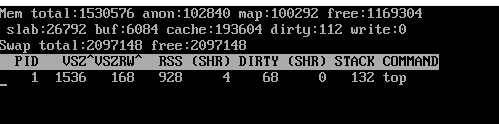
\includegraphics[width=\columnwidth]{./Figure/commands/pid-normal}
\end{column}
\begin{column}{.50\textwidth}
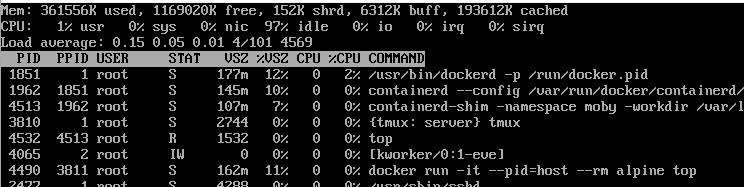
\includegraphics[width=\columnwidth]{./Figure/commands/pid-host}
\end{column}
\end{columns}
\end{frame}

\begin{frame}[fragile]
\frametitle{RUN}
\framesubtitle{limiting resources}
\begin{lstlisting}
$ docker run -dt --name vm -m 1g ubuntu:18.04 /bin/bash
\end{lstlisting}
\begin{itemize}
\item \lstinline!-m! max amount of memory available
\item \lstinline!--memory-swap! max amount of swap memory. If not specified is equal to the max memmory (in this case 1GB)
\item \lstinline!--cpus! number of cpus available. Can be a fraction
\end{itemize}
\end{frame}

\begin{frame}[fragile]
\frametitle{RUN}
\framesubtitle{command arguments}
\begin{lstlisting}
$ docker run -t  -m 1g ubuntu:18.04 ls -lph /var
\end{lstlisting}
Just place them after the command.
\end{frame}

\begin{frame}[fragile]
\frametitle{RUN}
\framesubtitle{environment}
\begin{lstlisting}
$ docker run -it -e "DEBUG=true" ubuntu:18.04 ls -lph /
\end{lstlisting}
Set the value of an environment variable.\\
\vspace{0.4cm}
A separate \lstinline!-e! for each variable.
\end{frame}

\begin{frame}[fragile]
\frametitle{RUN}
\framesubtitle{Detach from a running container}
\begin{lstlisting}
$ docker run --rm -it --name Duck ubuntu:18.04 /bin/bash
\end{lstlisting}
Detach from the container using \lstinline!Ctrl-P! + \lstinline!Ctrl-Q!
\end{frame}

\begin{frame}[fragile]
\frametitle{RUN}
\framesubtitle{ReAttach to a running container}
\begin{lstlisting}
$ docker attach Duck
\end{lstlisting}
\end{frame}

\begin{frame}[fragile]
\frametitle{Processes}
\scriptsize
\begin{lstlisting}[breaklines=true]
$ docker ps --help

Usage:  docker ps [OPTIONS]

List containers

Options:
  -a, --all             Show all containers (default shows just running)
  -f, --filter filter   Filter output based on conditions provided
      --format string   Pretty-print containers using a Go template
  -n, --last int        Show n last created containers (includes all states) (default -1)
  -l, --latest          Show the latest created container (includes all states)
      --no-trunc        Don't truncate output
  -q, --quiet           Only display numeric IDs
  -s, --size            Display total file sizes
\end{lstlisting}
\normalsize
\end{frame}

\begin{frame}[fragile]
\frametitle{Processes}
\begin{lstlisting}
$ docker ps
\end{lstlisting}
List the running containers 
\begin{lstlisting}
$ docker ps -a
\end{lstlisting}
List all containers 
\end{frame}


\begin{frame}[fragile]
\frametitle{RUN}
\framesubtitle{ReAttach to a running container}
Using the container \textit{id}
\end{frame}


\begin{frame}[fragile]
\frametitle{EXEC}
\scriptsize
\begin{lstlisting}[breaklines=true]
$ docker exec --help

Usage:  docker exec [OPTIONS] CONTAINER COMMAND [ARG...]

Run a command in a running container

Options:
  -d, --detach               Detached mode: run command in the background
      --detach-keys string   Override the key sequence for detaching a container
  -e, --env list             Set environment variables
  -i, --interactive          Keep STDIN open even if not attached
      --privileged           Give extended privileges to the command
  -t, --tty                  Allocate a pseudo-TTY
  -u, --user string          Username or UID (format: <name|uid>[:<group|gid>])
  -w, --workdir string       Working directory inside the container
\end{lstlisting}
\normalsize
\end{frame}

\begin{frame}[fragile]
\frametitle{EXEC}
\begin{lstlisting}
$ docker exec vm df -h
\end{lstlisting}

Runs a command (in this case \lstinline!df -h!) in a running container
\end{frame}

\begin{frame}[fragile]
\frametitle{IMAGES}
\scriptsize
\begin{lstlisting}[breaklines=true]
$ docker images --help

Usage:  docker images [OPTIONS] [REPOSITORY[:TAG]]

List images

Options:
  -a, --all             Show all images (default hides intermediate images)
      --digests         Show digests
  -f, --filter filter   Filter output based on conditions provided
      --format string   Pretty-print images using a Go template
      --no-trunc        Don't truncate output
  -q, --quiet           Only show numeric IDs
\end{lstlisting}
\normalsize
\end{frame}


\begin{frame}[fragile]
\frametitle{IMAGES}
\begin{lstlisting}
$ docker images
\end{lstlisting}

List the images 
\end{frame}

\begin{frame}[fragile]
\frametitle{IMAGE}
\scriptsize
\begin{lstlisting}[breaklines=true]
$ docker image --help

Usage:  docker image COMMAND
Manage images

Options:

Commands:
  build       Build an image from a Dockerfile
  history     Show the history of an image
  import      Import the contents from a tarball to create a filesystem image
  inspect     Display detailed information on one or more images
  load        Load an image from a tar archive or STDIN
  ls          List images
  prune       Remove unused images
  pull        Pull an image or a repository from a registry
  push        Push an image or a repository to a registry
  rm          Remove one or more images
  save        Save one or more images to a tar archive (streamed to STDOUT by default)
  tag         Create a tag TARGET_IMAGE that refers to SOURCE_IMAGE

Run 'docker image COMMAND --help' for more information on a command.
\end{lstlisting}
\normalsize
\end{frame}

\begin{frame}[fragile]
\frametitle{IMAGE}
\framesubtitle{inspect}
\begin{lstlisting}
$ docker image inspect hello-world
\end{lstlisting}

Gives several information on the image
\end{frame}


\begin{frame}[fragile]
\frametitle{Remove Image}
\begin{lstlisting}
$ docker rmi hello-world
\end{lstlisting}

Deletes a local image. It has no effect on the hub.
\end{frame}

\begin{frame}[fragile]
\frametitle{Remove container}
\scriptsize
\begin{lstlisting}[breaklines=true]
$ docker rm --help

Usage:  docker rm [OPTIONS] CONTAINER [CONTAINER...]

Remove one or more containers

Options:
  -f, --force     Force the removal of a running container (uses SIGKILL)
  -l, --link      Remove the specified link
  -v, --volumes   Remove the volumes associated with the container
\end{lstlisting}
\normalsize
\end{frame}

\begin{frame}[fragile]
\frametitle{Remove container}
\begin{lstlisting}
$ docker rm vm
\end{lstlisting}
Deletes a container and all its data (volumes) 
\end{frame}

\begin{frame}[fragile]
\frametitle{System pruning}
\begin{lstlisting}
$ docker system prune
\end{lstlisting}

Reclaim all disk space
\end{frame}

\begin{frame}[fragile]
\frametitle{System}
\scriptsize
\begin{lstlisting}[breaklines=true]
$ docker system --help

Usage:  docker system COMMAND
Manage Docker
Options:

Commands:
  df          Show docker disk usage
  events      Get real time events from the server
  info        Display system-wide information
  prune       Remove unused data

Run 'docker system COMMAND --help' for more information on a command.
\end{lstlisting}
\normalsize
\end{frame}

\begin{frame}[fragile]
\frametitle{Disk space}
\begin{lstlisting}
$ docker system df
\end{lstlisting}
Shows what is using disk space
\end{frame}

\begin{frame}[fragile]
\frametitle{PULL}
\scriptsize
\begin{lstlisting}[breaklines=true]
$ docker pull --help

Usage:  docker pull [OPTIONS] NAME[:TAG|@DIGEST]

Pull an image or a repository from a registry

Options:
  -a, --all-tags                Download all tagged images in the repository
      --disable-content-trust   Skip image verification (default true)
\end{lstlisting}
\normalsize
\end{frame}

\begin{frame}[fragile]
\frametitle{PULL}
\begin{lstlisting}
$ docker pull ubuntu:14.08
\end{lstlisting}

Download from the public repository a desired image
\end{frame}

\begin{frame}[fragile]
\frametitle{COMMIT}
Transforming a container into an image.
\begin{itemize}
\item run a container w/o \lstinline!--rm!
\item install some software
\item exit from the container
\item remember the container id
\item commit the change.
\end{itemize}
\end{frame}

\begin{frame}[fragile]
\frametitle{COMMIT}
\framesubtitle{Transform a container into an image.}
\scriptsize
\begin{lstlisting}[breaklines=true]
$ docker commit --help
Usage:  docker commit [OPTIONS] CONTAINER [REPOSITORY[:TAG]]

Create a new image from a container s changes

Options:
  -a, --author string      Author (e.g., John Hannibal Smith <hannibal@a-team.com>)
  -c, --change list         Apply Dockerfile instruction to the created image
  -m, --message string Commit message
  -p, --pause                Pause container during commit (default true)
\end{lstlisting}
\normalsize
\end{frame}

\begin{frame}[fragile]
\frametitle{COMMIT}
\framesubtitle{Transform a container into an image.}
\scriptsize
\begin{lstlisting}[breaklines=true]
$ docker run -it ubuntu:18.04 sh -c apt update && apt install git

$ docker ps -a
CONTAINER ID  IMAGE           COMMAND                  NAMES
8bb0b797af88   ubuntu:18.04 sh -c ''apt update''       condescending_shaw

$ docker commit -m install git 8bb0b797af88 ubuntu_git:0.1
sha256:c47472e998a05687938fc9a5ebfa6cfbfff137aeb360b37de00e99515ab0298a

$ docker images | head
REPOSITORY  TAG IMAGE ID         SIZE
ubuntu_git      0.1  c47472e998a0 212MB
\end{lstlisting}
\normalsize
\end{frame}